\chapter{Quick Start}
\label{ch:quickstart}

\newthought{Ten minutes from install to results.} This chapter runs a complete scan with
nothing but the packages you installed in Chapter~\ref{ch:installation}: twenty random
points through a built-in test operator, archived into \textsc{hdf5} and \textsc{csv}. It
then tours the output tree and shows the two commands you will reach for next ---
\cli{Jarvis2 monitor} and \cli{Jarvis2 project}.

\section{Before you start}

Make sure Redis is up:

\begin{terminal}
\begin{jcmd}
redis-cli ping        # -> PONG
\end{jcmd}
\end{terminal}

\section{The task card}
\label{sec:quickstart-card}

Save the following as \file{quickstart.yaml} in any directory. Outputs will land in
\file{<project-root>/outputs/<scan-name>/} next to it.\sidenote{Without an explicit
project marker, the directory containing the task card becomes the project root ---
Chapter~\ref{ch:core-concepts} has the exact resolution rules.}

\begin{yamlwin}
project_name: quickstart
Scan:
  name: quickstart

EnvReqs:
  V2:
    workers: 2                # two Worker processes
    batch_size: 256           # sampler submit-group size

Sampling:
  Method: Random
  "Point number": 20          # note: the key contains a space
  Seed: 7
  Variables:
    - name: x
      distribution: {type: Flat, parameters: {min: 0.0, max: 1.0}}
    - name: y
      distribution: {type: Flat, parameters: {min: 0.0, max: 1.0}}
  LogLikelihood:
    - name: LogL_Z
      expression: z

Operas:
  Modules:
    - name: TrivialEggbox
      operator: jarvishep2.testing.eggbox.eggbox2d_numpy
      call_mode: call
      input:
        - {name: x, expression: x}
        - {name: y, expression: y}
      output:
        - {name: z, entry: z}
\end{yamlwin}

Reading it top to bottom:

\begin{itemize}
  \item \yamlkey{Scan.name} names the scan and its output directory.
  \item \yamlkey{EnvReqs.V2} is the only scheduling block: how many Workers, and how many
        tasks the sampler pushes to Redis per group (Chapter~\ref{ch:envreqs}).
  \item \yamlkey{Sampling} picks the \sampler{Random} method, a budget of twenty points, a
        seed, and two flat variables $x,y\in[0,1]$ (Chapters~\ref{ch:sampling-block}
        and~\ref{ch:variables}).
  \item \yamlkey{Operas.Modules} declares one in-process operator --- a test
        \emph{eggbox} function shipped with the runtime --- fed by the expressions
        \expr{x} and \expr{y}, returning one observable \code{z}
        (Chapter~\ref{ch:operas}).
  \item \yamlkey{Sampling.LogLikelihood} scores every point with the expression \expr{z}
        (Chapter~\ref{ch:loglikelihood}).
\end{itemize}

No external programs, no input files: the whole workflow runs inside the Workers.

\section{Run it}
\label{sec:quickstart-run}

\begin{terminal}
\begin{jcmd}
Jarvis2 run quickstart.yaml
\end{jcmd}
\end{terminal}

\cli{Jarvis2 run} loads and validates the card, starts the managed processes, submits
the twenty points, and shuts everything down once the last Sample is archived. Every
managed process is named \code{<role>:\allowbreak{}quickstart} in \cli{ps}/\cli{top} ---
\code{Jarvis2}, \code{Jarvis2-\allowbreak{}Worker-\allowbreak{}1},
\code{Jarvis2-\allowbreak{}Worker-\allowbreak{}2},
\code{Jarvis2-\allowbreak{}Archiver}, and \code{Jarvis-\allowbreak{}Redis} if it
started that too --- so the scan
stays identifiable even with several running at once. The console ends with a
\code{[Scan Performance]} block: wall time, \code{samples / sec}, average time per
sample.

\begin{jtip}
Stop a running scan with \textbf{Ctrl+C}. \Jtwo\ catches the interrupt and shuts down
Workers, the Archiver, and any Redis it started. Avoid \textbf{Ctrl+Z}: suspending leaves
the process group half-alive, so \Jtwo\ ignores it during a scan.
\end{jtip}

Exit codes are meaningful in scripts: \code{0} all samples succeeded, \code{1} any sample
failed (including partial failure) or a runtime error, \code{2} a usage or configuration
error, \code{130} interrupted.

\section{What you got}
\label{sec:quickstart-outputs}

\begin{jfiletree}
\dirtree{%
.1 \dtfoldopen{outputs/quickstart/}.
.2 \dtfoldopen{DATABASE/}.
.3 \dtdata{samples.hdf5}\DTcomment{one record per Sample}.
.3 \dtcsv{samples.csv}\DTcomment{full-column export}.
.2 \dtfold{SAMPLE/}\DTcomment{per-sample artifacts (empty here)}.
.2 \dtjson{run\_summary.json}.
.2 \dtcsv{run\_summary.csv}.
.2 \dtdoc{run\_summary.txt}.
}
\end{jfiletree}

\begin{itemize}
  \item \file{DATABASE/samples.hdf5} holds one record per Sample: the parameters
        \code{x}, \code{y}, the observable \code{z}, and \code{LogL}
        (Chapter~\ref{ch:outputs}).
  \item \file{DATABASE/samples.csv} is a full-column export of the same records --- open
        it in anything.
  \item \file{SAMPLE/} holds per-sample artifact directories; for this opera-only scan
        with nothing saved, they stay empty and out of the way.
  \item \file{run\_summary.*} record counters and throughput in three formats
        (Chapter~\ref{ch:monitoring}).
\end{itemize}

Logs live under \file{logs/}: a control log per scan, one log for the Archiver, and one
per Worker (Chapter~\ref{ch:logging}).

A quick look at the results:

\begin{terminal}
\begin{jcmd}
python3 - <<'PY'
import pandas as pd
df = pd.read_csv("outputs/quickstart/DATABASE/samples.csv")
print(df[["x", "y", "z", "LogL"]].head())
PY
\end{jcmd}
\end{terminal}

\section{The black-box model}
\label{sec:quickstart-blackbox}

\newthought{What you just ran is the easy case.} \yamlkey{Operas.Modules} calls a
Python function that already lives inside the Worker process --- no file, no
subprocess, nothing to install. Most real physics work is not that: it means driving a
spectrum generator, a dark-matter code, a recasting tool, or your own analysis script
--- a program you did not write for \Jtwo\ and have no reason to rewrite.

\Jtwo's answer is to treat that program as a \textbf{black box}. It never reads your
program's source or knows what language it is written in; for every point it only
does three things, in order:

\begin{enumerate}
  \item \textbf{Write one input file}, from the sampled parameters.
  \item \textbf{Run the program's own command} exactly as you would from a shell.
  \item \textbf{Read one output file} back, and keep the values you asked for.
\end{enumerate}

That is the entire contract. On a Unix system everything is a file and every program
is a black box already --- \Jtwo\ just automates opening it, over and over, once per
Sample. Whether the box is a hundred-line Fortran spectrum generator or the four-line
Python script below, the recipe never changes. The rest of this section builds one,
block by block, using the \emph{same} \code{z = (sin(x) * cos(y) + 2) ** 5} physics as
the card above (Figure~\ref{fig:eggbox-landscape}). Compare the two side by side and
see exactly what changes when the calculation moves outside Python.

\begin{jtip}
Before writing any of this, answer four questions: \emph{which parameters am I
scanning}, \emph{which program computes my observables}, \emph{which output values do
I actually need}, and \emph{what likelihood judges them}. For this example: \code{x},
\code{y}; the \file{eggbox.\allowbreak{}py} script below; one value, \code{z}; and
\expr{LogGauss(z, 100, 10)} --- a stand-in ``experiment'' that measures
$z = 100 \pm 10$.
\end{jtip}

\begin{fullwidth}
\begin{figure}[ht]
\centering
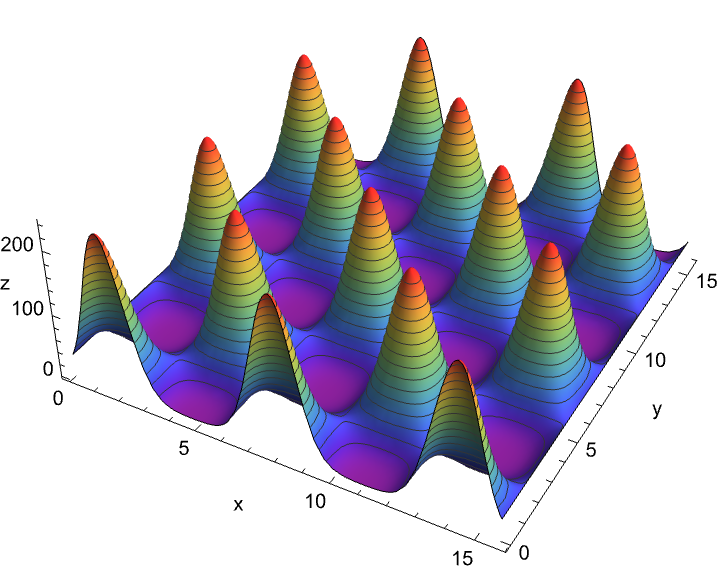
\includegraphics[width=0.7\linewidth]{figures/eggbox_vis.png}
\caption[The eggbox landscape.]{$z(x,y) = (\sin x\cos y + 2)^5$ over the scan range ---
the repeating peaks and valleys are why the function (and this tutorial) is called
\emph{eggbox}. The scan's job is to find where this surface sits inside the target
band $z = 100 \pm 10$; \sampler{Bridson} covers the $(x,y)$ plane below, and every
peak/valley the sampler lands on becomes one Sample.}
\label{fig:eggbox-landscape}
\end{figure}
\end{fullwidth}

\section{Building a black-box card, block by block}
\label{sec:quickstart-card2}

\paragraph{\yamlkey{Scan}: name and layout.}

\begin{yamlwin}
Scan:
  name: "EggBox_Bridson"
  save_dir: "&J/outputs"
\end{yamlwin}

Same key as the first card's \yamlkey{Scan.name}; \yamlkey{save\_dir} just makes the
output root explicit instead of relying on the default (Chapter~\ref{ch:task-yaml}).

\paragraph{\yamlkey{Sampling}: the scan geometry.}

\begin{yamlwin}
Sampling:
  Method: "Bridson"
  Variables:
    - name: x
      description: "Variable X."
      distribution: {type: Log, parameters: {min: 0.1, max: 5.0, length: 1.0}}
    - name: y
      description: "Variable Y."
      distribution: {type: Flat, parameters: {min: 0.0, max: 5.0, length: 1.0}}
  Radius: 1
  MaxAttempt: 30
  LogLikelihood:
    - {name: "LogL_Z", expression: "LogGauss(z, 100, 10)"}
\end{yamlwin}

\sampler{Bridson} instead of \sampler{Random} this time (Chapter~\ref{ch:bridson}) ---
\yamlkey{Radius} and \yamlkey{MaxAttempt} are its two required keys, and every
variable needs a \yamlkey{length} for the blue-noise geometry. \yamlkey{LogLikelihood}
is the same shape as before, now scoring the observable this card's calculator will
produce.

\paragraph{\yamlkey{EnvReqs}: the runtime floor.}

\begin{yamlwin}
EnvReqs:
  OS:
    - {name: linux, version: ">=3.10.0"}
    - {name: Darwin, version: ">=10.0"}
  Check_default_dependencies:
    required: true
    default_yaml_path: "&J/deps/environment_default.yaml"
\end{yamlwin}

\yamlkey{OS} is descriptive metadata --- \Jtwo\ preserves it but does not enforce it
at load time (Chapter~\ref{ch:envreqs}). \yamlkey{Check\_default\_dependencies} is the
part that does something: it merges a shared defaults file's \yamlkey{EnvReqs.V2} map
under this card's own, so a whole project can keep one common runtime configuration
instead of repeating \yamlkey{workers} / \yamlkey{batch\_size} on every card
(Section~\ref{sec:check-default-deps}).

\paragraph{\yamlkey{Calculators}: the black box itself.} This is the part most users
actually need to learn --- everything above just sets the stage.

\begin{yamlwin}
Calculators:
  make_paraller: 4
  path: "&J/calculators/runtime/program"
  Modules:
    - name: EggBox
      clone_shadow: true
      source: "&J/deps/assets/inertial/EggBox"
      path: "&J/calculators/runtime/program/EggBox/@PackID"
      installation:
        - "cp -r ${source}/* ${path}"
      initialization:
        - "cp ${source}/input.json ${path}/input.json"
        - "rm -f ${path}/output.json"
      execution:
        path: "&J/calculators/runtime/program/EggBox/@PackID"
        commands:
          - "./eggbox.py"
        input:
          - name: inpjson
            path: "&J/calculators/runtime/program/EggBox/@PackID/input.json"
            type: JSON
            save: false
            actions:
              - type: Dump
                variables:
                  - {name: xx, expression: "x * Pi"}
                  - {name: yy, expression: "y * Pi"}
        output:
          - name: oupjson
            path: "&J/calculators/runtime/program/EggBox/@PackID/output.json"
            type: JSON
            save: true
            variables:
              - {name: z}
\end{yamlwin}

Field by field:

\begin{itemize}
  \item \yamlkey{make\_paraller} --- how many parallel calculator slots exist across
        all Workers (the spelling is historical, Chapter~\ref{ch:calculators}).
  \item \yamlkey{clone\_shadow: true} --- every concurrent Sample gets its own physical
        copy of the program directory, so two Samples never fight over the same
        \file{input.json}; \token{@PackID} is the slot identifier that makes each copy's
        path unique (Section~\ref{sec:clone-shadow}).
  \item \yamlkey{source} --- where the program template lives; \yamlkey{path} --- where
        \Jtwo\ stages a working copy of it.
  \item \yamlkey{installation} --- runs \emph{once per pack}: stage the program
        (\code{cp -r \$\{source\}/* \$\{path\}}).
  \item \yamlkey{initialization} --- runs before every point: drop a fresh
        \file{input.\allowbreak{}json} template and clear any leftover
        \file{output.\allowbreak{}json} from the previous point.
  \item \yamlkey{execution.commands} --- the actual shell command, run from
        \yamlkey{execution.path}: exactly \code{./eggbox.py}, as if you had typed it
        yourself.
  \item \yamlkey{execution.input} --- how to \emph{write} the input file: \yamlkey{type:
        JSON}, action \yamlkey{Dump}, and a \yamlkey{variables} list mapping the sampled
        \code{x}/\code{y} to the JSON fields the script expects, \code{xx}/\code{yy}
        (multiplied by $\pi$, matching \file{eggbox.py}'s own convention).
  \item \yamlkey{execution.output} --- how to \emph{read} the output file back: the
        same \yamlkey{type: JSON}, and one variable, \code{z}, copied straight from the
        JSON field of the same name into the observables dictionary.
\end{itemize}

\begin{jnote}
Nothing above is eggbox-specific. Swap \yamlkey{source}/\yamlkey{path} for your own
tool, \yamlkey{execution.commands} for however you actually invoke it, and
\yamlkey{type: JSON} for whatever format it reads and writes (\textsc{slha}, plain
text, \ldots --- Chapter~\ref{ch:io-types} has every format \Portal\ supports). The
shape --- install once, initialize per point, run, read output --- never changes.
\end{jnote}

\section{Run it}
\label{sec:quickstart-run2}

\begin{terminal}
\begin{jcmd}
Jarvis2 run bin/Example_Bridson_process.yaml
\end{jcmd}
\end{terminal}

\begin{jtip}
Do not type the card above by hand to try it: \cli{Jarvis2 project fetch Eggbox}
(Section~\ref{sec:quickstart-project}) downloads it complete and runnable, as
\file{bin/Example\_Bridson\_process.yaml}, right beside
\file{bin/Example\_Bridson\_Operas.yaml} --- the Operas version you ran earlier. Diff
the two files to see, line for line, exactly what changes when the physics moves
outside Python.
\end{jtip}

\section{Adapting this to your own physics case}
\label{sec:quickstart-adapt}

Five things change between this toy and a real model; nothing else does:

\begin{enumerate}
  \item \textbf{The parameters.} In \yamlkey{Sampling.Variables}, replace \code{x}/\code{y}
        with your own model's parameters --- \code{m0}, \code{m12}, \code{tanb},
        whatever your program takes --- and pick the distribution and range each one
        needs (Chapter~\ref{ch:variables}).
  \item \textbf{The calculator.} In \yamlkey{Calculators.Modules}, point \yamlkey{source}
        at your tool and rewrite \yamlkey{installation}/\yamlkey{initialization} for
        however it actually needs to be staged.
  \item \textbf{The input mapping.} In \yamlkey{execution.input}, match your tool's real
        input format (\yamlkey{type: SLHA} instead of \code{JSON}, for instance) and
        list the fields it expects, expressed in terms of your new parameters.
  \item \textbf{The output mapping.} In \yamlkey{execution.output}, list the physical
        quantities your tool actually produces --- masses, cross sections, branching
        ratios --- instead of \code{z}.
  \item \textbf{The likelihood.} In \yamlkey{Sampling.LogLikelihood}, replace
        \expr{LogGauss(z, 100, 10)} with an expression over the observables your
        calculator's \yamlkey{output} now produces (Chapter~\ref{ch:loglikelihood}).
\end{enumerate}

\begin{jtip}
Once these five are consistent with each other --- every observable your likelihood
names is actually produced by \yamlkey{execution.output} --- \Jtwo\ can run the scan.
Everything else in this chapter (running, monitoring, outputs) works identically
whether the workflow behind it is one Python function or ten external programs in
five dependency layers.
\end{jtip}

\section{Watching a longer scan}
\label{sec:quickstart-monitor}

Twenty points finish before you can look up. For a real scan, open a second terminal and
attach the read-only monitor:

\begin{terminal}
\begin{jcmd}
Jarvis2 monitor
\end{jcmd}
\end{terminal}

It prints one snapshot --- Workers alive, queue lengths, samples running/completed/failed,
calculator slots --- and exits. It never writes to Redis, so it is always safe
(Chapter~\ref{ch:monitoring}).

\begin{jtip}
On a scan that runs for hours, you do not have to wait for it to finish to look at
results: \cli{Jarvis2 convert <task>.yaml} re-derives \file{samples.csv} from whatever
the Archiver has flushed to \textsc{hdf5} so far, in a second terminal, without
touching the running scan (Section~\ref{sec:cli-convert}).
\end{jtip}

\section{Starting from a scaffold instead}
\label{sec:quickstart-project}

Rather than a bare \textsc{yaml} in a directory, you can let \Jtwo\ scaffold a proper
project, or fetch a complete example from the official catalog:

\begin{terminal}
\begin{jcmd}
# a fresh project with a ready-to-run card
Jarvis2 project create MyScan
cd MyScan
Jarvis2 run bin/quickstart_bridson_operas.yaml

# or browse and fetch official examples
Jarvis2 project list
Jarvis2 project fetch Eggbox
\end{jcmd}
\end{terminal}

Chapter~\ref{ch:project-cli} covers the project tools, the catalog, and how to pack and
share your own projects.

\section{Where to go next}

\begin{itemize}
  \item The vocabulary behind what just happened --- projects, tokens, u-space, Samples,
        buckets --- is Chapter~\ref{ch:core-concepts}.
  \item To point the same skeleton at a \emph{real} external program, read the
        calculator chapters (Chapters~\ref{ch:workflow-model}--\ref{ch:io-types}).
  \item To choose a smarter sampler than \sampler{Random}, start at
        Chapter~\ref{ch:choosing-sampler}.
  \item To see \file{samples.csv} as a figure instead of a \code{pandas} table,
        Chapter~\ref{ch:jarvisplot} covers \cli{Jarvis2 plot}.
\end{itemize}
